\chapter{February}

\section{Feb 1st}\index{Feb 1st}
\subsection{Standard deviation} \index{Standard deviation}
\textbf{Standard deviation} $\sigma$ is defined as the square root of \textbf{variance}. That is,
\begin{align}
	\sigma(X) &= \sqrt{var(X)}
\end{align}
The definition for variance:
\begin{align}
var(X) = E[(X - \mu_X)^2]
\end{align}
The definition for \textbf{covariance}:
\begin{align}
cov(X,Y) = E[(X - \mu_X)(Y- \mu_Y)]
\end{align}
A property:
\begin{align}
	cov(X,X) = var(X) = \sigma(X)^2 
\end{align}
Definition for \textbf{correlation}:
\begin{align}
	\begin{split}
	\rho(X,Y) & = corr(X, Y) 		\\
			  & = \frac{cov(X,Y)}{\sigma_X \sigma_Y}
	\end{split}
\end{align}

\section{Feb 2nd}\index{Feb 2nd}

\subsection{Determinant}\index{Determinant}
Today when I try to compute the determinant of the covariance matrix in the multivariate Gaussian, I come across the problem of overflow. In fact, I only
need to know the logarithm of the determinant. Therefore, I apply the following solution:
\begin{align}
	\begin{split}
	\log(\det A) &= \log(\Pi_{i=1}^{N} \lambda_i)  \\
				 & = \sum_{i=1}^{N} \log(\lambda_i)
	\end{split}
\end{align}

\subsection{Matplotlib}\index{Matplotlib}
Sample code to plot figures with Python:

\begin{minted}[frame=lines, framesep=2mm,]
	       {python}
x = np.linspace(-10, 4, 500, endpoint=True)
y = (3 * x + 12) / 4

fig = plt.figure()
fig.suptitle('Problem 3', fontsize=20, fontweight='bold')
ax = fig.add_subplot(111)
ax.plot(x, y)

ax.spines['right'].set_color('none')
ax.spines['top'].set_color('none')
ax.xaxis.set_ticks_position('bottom')
ax.spines['bottom'].set_position(('data',0))
ax.yaxis.set_ticks_position('left')
ax.spines['left'].set_position(('data',0))

plt.annotate(r'$(-4,0)$',
xy=(-4, 0), xycoords='data',
xytext=(-20, +60), textcoords='offset points', fontsize=16,
arrowprops=dict(arrowstyle="->", connectionstyle="arc3,rad=.2"))

plt.annotate(r'$(0,3)$',
xy=(0, 3), xycoords='data',
xytext=(+10, -30), textcoords='offset points', fontsize=16,
arrowprops=dict(arrowstyle="->", connectionstyle="arc3,rad=.2"))

plt.annotate(r'positive',
xy=(-6, 2), xycoords='data',
xytext=(+10, +30), textcoords='offset points', fontsize=16)

ax.set_xlabel("x")
ax.set_ylabel("y")

plt.savefig('3.png', dpi = 100)
plt.show()
\end{minted}

\section{Feb 3rd}\index{Feb 2nd}
\subsection{Different types of machine learning methods:}
\begin{enumerate}
\item \textbf{Parametric methods}: a family of distributions that can be described using a finite 
number of paramters, such as \textit{GMM, Naive Bayes, SVM}.
\item \textbf{Non-parametric methods}: methods that are not based on parametrized families of
probability distributions, such as \textit{decision trees, KNN}. 
\end{enumerate}

The difference between parametric models and non-parametric models is that the former 
has a fixed number of parameters, while the latter grows the number of parameters with 
the amount of training data.
\begin{remark}
Note that the non-parametric model does not have no parameters: parameters are determined by the training data, not the model.
\end{remark}

Parametric models can also be categorized into \textbf{generative models} and 
\textbf{discriminative models}.
\begin{enumerate}
\item Generative models: Fit a probability distribution like a multivariate Gaussian to each class.
\item Approximate the boundaries between classes by simple functions.
\end{enumerate}

\subsection{Representation Learning}


\paragraph{Dimensionality Reduction and Denoising}
Given data in high-dimensional Euclidean space, project to a
low-dimensional linear subspace while retaining as much of the
signal as possible. 

\paragraph{Embedding and manifold learning}
Given data that lie in a non-Euclidean space, find an embedding into
Euclidean space that preserves as much of the geometry as possible.

\paragraph{Metric learning}
A metric $d$ should satisfy the following properties:
\begin{enumerate}
	\item $d(x, y) \geq 0$, non-negativity
	\item $d(x, y) = 0$ if and only if $x = y$
	\item $d(x, y) = d(y, x)$, symmetry
	\item $d(x, z) \leq d(x, y) + d(y, z)$, triangle inequality
\end{enumerate}

\subsection{Fast Nearest Neighbor Search}
\textbf{Locality sensitive hashing.}\hspace{0.2cm} Grouping points in space into \textit{buckets} based on some distance metric operating on the points. Points that are close to each other under the chosen metric are mapped to the same bucket with high probability.

\textbf{K-d tress.}\hspace{0.2cm} A space-partitioning data structure for organizing points in a k-dimensional space.

\begin{remark}
	Nearest neighbor is sensitive to noise.
\end{remark}

\subsection{Decision Trees}
\textbf{Node split.}\hspace{0.2cm} When to split a node, we need to decide which 
node to split. We have the following methods to measure the \textbf{uncertainty in prediction} $u(S)$:
\begin{itemize}
	\item \textit{Misclassification rate}: $min(p, 1-p)$, where $p$ is the fraction of positive points.
	\item \textit{Gini index}: $2p(1-p)$
	\item \textit{Entropy}: $-p\log p - (1-p)\log(1-p)$
\end{itemize}
We select the node split that can mostly reduce uncertainty (see Figure~\ref{fig:feb-dt-split}).
\begin{figure}[h]
	\centering{
		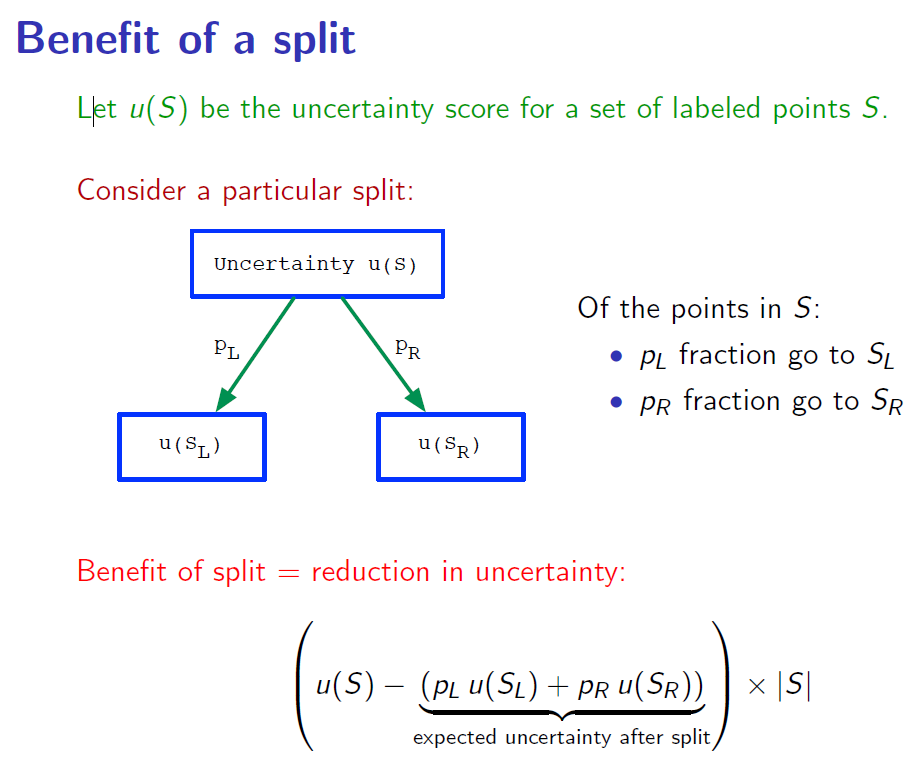
\includegraphics[width = 0.9\textwidth]{./images/feb/dt_split.PNG}
	}
	\label{fig:feb-dt-split}
	\caption{Benefit of a split.}
\end{figure} 


\textbf{When to stop?}\hspace{0.2cm} Keep splitting until leaves are pure. 

\textbf{Pruning.}\hspace{0.2cm} After split stops, we do pruning to avoid over-fitting. Consider all pairs of leave nodes,
any pair whose elimination yields a satisfactory (small)
increase in impurity is eliminated, and the common
antecedent node is declared as leaf node.

\subsection{Classification with generative models}

\textbf{Bayes-optimal prediction.}\hspace{0.2cm}
\begin{align}
	\begin{split}
	Pr(y= j | x) &= \frac{Pr(y= j) Pr(x|y=j)}{Pr(x)} \\
		&= \frac{\pi_j P_j(x)}{\sum_{i=1}^{k} \pi_i P_i(x)}
	\end{split}
\end{align}


\textbf{Laplace smoothing.}\hspace{0.2cm}
We want to estimate $p_{ji} = Pr(x_i = 1 | y=j)$. Then the maximum likelihood estimate of $p_{ji}$ is $p_{ij} = \frac{n_{ji}}{n_j}$, where $n_{ji}$ is the number of instances of class $j$ with $x_i = 1$, and $n_j$ is the number of 
instances of class $j$. 
\begin{remark}
This causes the problem if $n_{ji} = 0$. Instead, we use \textit{Laplace smoothing}: $p_{ji} = \frac{n_{ji} + 1}{n_j + 2}$
\end{remark} 


\textbf{Multinomial naive Bayes.}\hspace{0.2cm}
Classify document $x$ as $\argmax_j \pi_j \prod_{i=1}^{N} p_{ji} ^ {x_i}$.
To improve the performance, we may adopt the following heuristics:
\begin{itemize}
	\item Compensating for burstiness. Problem: once a word has appeared in a document, it has a much higher chance of appearing again.
	Solution: Instead of the number of occurrences $f$ of a word, use
	$\log(1 + f )$.
	
	\item Downweighting common words. Problem: common words can have a unduly large influence on classification. Solution: weight each word $w$ by \textit{inverse document frequency}:
	\[
		\log\frac{\# \text{docs}}{\#(\text{docs containing w})}
	\]
\end{itemize}

\subsection{Gaussian}
\textbf{Multivariate Gaussian.}\hspace{0.2cm} mean: $\mu \in R^p$. covariance $p\times p$
matrix $\sum$:
\begin{align}
\begin{split}
	p(x) &= \frac{1}{(2\pi)^{p/2} |\sum|^{1/2}} \exp(-\frac{1}{2} (x-\mu)^T \sum {}^{-1} (x-\mu))
\end{split}
\end{align}

\textbf{Spherical Gaussian.}\hspace{0.2cm} $\sum = diag(\sigma^2, ..., \sigma^2)$

\textbf{Diagonal Gaussian.}\hspace{0.2cm} $\sum = diag(\sigma_1^2, ..., \sigma_p^2)$




















